\documentclass{vldb}
\usepackage{graphicx}
\usepackage{balance}  % for  \balance command ON LAST PAGE  (only there!)
\newtheorem{example}{Example}

\begin{document}

% ****************** TITLE ****************************************

\title{QOCO-R:Query and Rules Oriented Data Cleaning}

% ****************** AUTHORS **************************************

\numberofauthors{3}

\author{
% 1st. author
\alignauthor
Ahmad Assadi\\
%       \affaddr{Tel-Aviv University}\\
%       \email{trovato@corporation.com}
% 2nd. author
\alignauthor
Tova Milo\\
%       \affaddr{Tel-Aviv University}\\
%       \email{webmaster@marysville-ohio.com}
% 3rd. author
\alignauthor 
Slava Novgorodov\\
%       \affaddr{Tel-Aviv University}\\
%       \email{larst@affiliation.org}
}
\maketitle


\begin{abstract}
Fill Content
\end{abstract}

\section{Introduction}
Fill intro

\section{Rules}
The rules in QOCO-R are a database assertions that delivered to the algorithm by the Oracle. In order to get an effective rules language it must enable expressing all popular relational database assertions. As in \cite{queryreformulation,dataexchange} The embedded dependencies include all of the naturally-occurring constraints on relational databases. They are a first order logic formulas of the form:
\begin{center}
$\mathtt{\forall x_{1},...,x_{n} \phi(x_{1},...,x_{n}) \rightarrow \exists z_{1},...,z_{m} \psi(x_{1},...,x_{n},z_{1},...,z_{m}) }$
\end{center}
where the left hand side (LHS) of the implication, $\phi$, is a conjunction
of relational formulas over variables $\bar{x}$, and the right hand side (RHS)
of the implication, $\psi$, is a conjunction of relational or equality formulas over variables $\bar{x}$
and $\bar{z}$.\\
The embedded dependencies is comprised of tuple-generating dependencies (tgds) of the form:
\begin{center}
$\mathtt{\forall x_{1},...,x_{n} \phi(x_{1},...,x_{n}) \rightarrow \exists z_{1},...,z_{m} R(x_{1},...,x_{n},z_{1},...,z_{m}) }$
\end{center}
and equality generating dependencies (egds) of the form:
\begin{center}
$\mathtt{\forall x_{1},...,x_{n} \phi(x_{1},...,x_{n}) \rightarrow x_{i} = x_{j} }$
\end{center}

In tgds the RHS contains only relational formulas and in egds the RHS contains only equality formulas. Given a particular combination of tuples satisfying the constraint of the LHS, tgds expresses an assertion about the existence of a tuple in the instance on the RHS,and egds expresses an assertion about an equality between two variables.\\
As we mentioned above our rules language should enable expressing tgds and egds, therefor the rules language consists of two sets of rules:
\begin{enumerate}
\item Tuple-generating rules (tgrs). They have the same form as tgds but the LHS may contain also constraints on variables (not only relational formulas), a constraint is a boolean expression of the form $v \, OP \, w$ where $v,w \in {\bar{x}}\cup \mathcal{C}$ and $OP$ is a boolean operation that defined on the variables domain, for example if $v$ and $w$ value should be a number then $OP$ should be $=,\neq,\leq,\geq,...$ \\
For    
\item Condition-generating rules (cgrs). They have the same form as egds but both the LHS and the RHS could contain a conjunction of constraints. 
\end{enumerate}  

\begin{example}
Consider the database in Figure \ref{fig:db} which shows portions of two relations of a football league. The Games relation describes the results of a match between two teams, it stores the teams name, goals score and penalties score. The Teams relation  describes a football team, it stores the team name and country. This database must satisfy the facts: (i) If a game ends with a draw then the penalties stage must determine the winner (ii) The team name uniquely determines it's country (iii) team1 column in Games relation should be included in name column in the Teams relation. Those facts are equal to the following rules: 
\begin{itemize}
\item $\mathtt{\forall \bar{x} \, Games(x_{1},x_{2},x_{3},x_{4},x_{5},x_{6}) \wedge x_{3}=x_{4} \rightarrow x_{5} \geq 0 \wedge x_{6} \geq 0 \wedge x_{5} \neq x_{6}  }$
\item $\mathtt{\forall \bar{x} \, Teams(x_{1},x_{2}) \wedge Teams(x_{3},x_{4}) \wedge x_{1}=x_{3} \rightarrow x_{2}=x_{4}}$
\item $\mathtt{\forall \bar{x} \, Games(x_{1},x_{2},x_{3},x_{4},x_{5},x_{6}) \rightarrow \exists \bar{z} \, Teams(x_{1},z_{1})}$
\end{itemize}
respectively where the first two are cgrs and the third is a tgr.
\end{example}

\begin{figure}
\centering
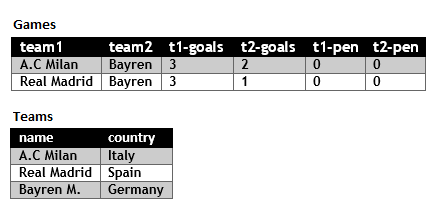
\includegraphics[width=9cm, height=4.5cm]{figure1}
\caption{Portion of a football league database.}
\label{fig:db}
\end{figure}

\section{System architecture}
Query and Rules Oriented Data Cleaning (QOCO-R) System comprises of 3 major blocks: Manager, Deletion module and insertion module, as shown in Figure \ref{fig:framework}.
The QOCO-R's input is a relational database \textit{D} where \textit{D} can contain invalid or missing data. The system has a user interface for enabling interaction with the crowd (oracles) and the users. As in QOCO, through the UI the user can specify two target actions: (i) remove a wrong answer from \textit{Q}(\textit{D}) or, (2) add a
missing answer to \textit{Q}(\textit{D})

\begin{figure}
\centering
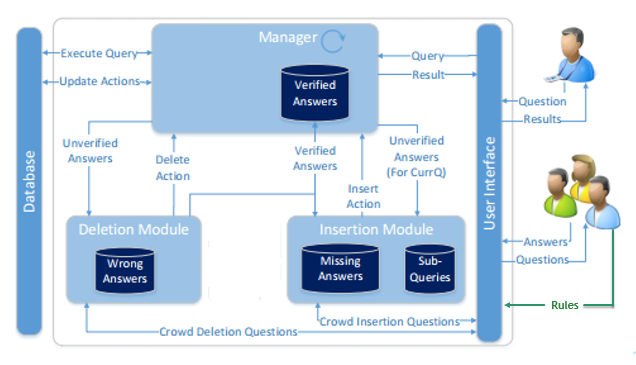
\includegraphics[width=9cm, height=4.5cm]{figure2}
\caption{QOCO-R framework architecture.}
\label{fig:framework}
\end{figure}
\section{Conclusions}
Content

%ACKNOWLEDGMENTS are optional
\section{Acknowledgments}
Content



\bibliographystyle{abbrv}
\bibliography{vldb_sample}  

\begin{thebibliography}{9}
\bibitem{queryreformulation} 
A. Deutsch, L.Popa, and V. Tannen. 
\textit{
Query reformulation with constraints. SIGMOD Record, 35(1), 2006}. 

\bibitem{dataexchange} 
R. Fagin, P. Kolaitis, R. J. Miller, , and L. Popa.
\textit{
Data exchange: Semantics and query answering. Theoretical Computer Science, 336, 2005}.
 
\end{thebibliography}

%APPENDIX is optional.
% ****************** APPENDIX **************************************
% Example of an appendix; typically would start on a new page
%pagebreak

\begin{appendix}
Content 

\end{appendix}



\end{document}
